% ==================================================================================================================================
% Introduction

\minitoc

Les fonctions sont des objets essentiels en mathématiques. Outre leur utilité dans des domaines appliqués, elles constituent des objets mathématiques passionnants. Leur étude permet non seulement de comprendre la transformation d’éléments d’un ensemble à un autre, mais aussi de manipuler des ensembles et des relations abstraites. Dans ce cours, nous utiliserons les termes \emph{fonctions} et \emph{applications} de manière interchangeable.

% ==================================================================================================================================
% Définition et notations 

\section{Définition et notations}

Une fonction peut être vue de deux façons différentes. La première la considère comme une sorte d’entité qui permet de « transformer » une valeur ou un élément en un autre. La seconde, que nous adopterons ici, la représente comme une correspondance entre deux ensembles.

\begin{definition}[Application]
    Soient $E$ et $F$ deux ensembles. Une fonction $f$ de $E$ vers $F$ est une correspondance qui à tout élément $x$ de $E$ associe un \textbf{unique} élément de $F$, noté $f(x)$. On écrit alors : 
    \[
        f : 
        \begin{cases}
            E \longrightarrow F \\ 
            x \longmapsto f(x)
        \end{cases}
    \]
\end{definition}

\begin{figure}[h!]
    \centering
    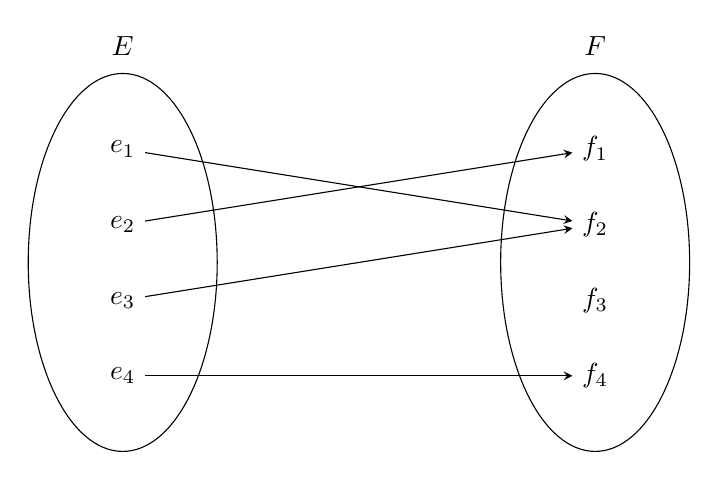
\begin{tikzpicture}[scale=1.2, >=stealth]
        % Ensembles
        \draw (0,0) ellipse (1 and 2) node[above=2.5cm] {$E$};
        \draw (5,0) ellipse (1 and 2) node[above=2.5cm] {$F$};

        % Points dans E
        \node (e1) at (0,1.2) {$e_1$};
        \node (e2) at (0,0.4) {$e_2$};
        \node (e3) at (0,-0.4) {$e_3$};
        \node (e4) at (0,-1.2) {$e_4$};

        % Points dans F
        \node (f1) at (5,1.2) {$f_1$};
        \node (f2) at (5,0.4) {$f_2$};
        \node (f3) at (5,-0.4) {$f_3$};
        \node (f4) at (5,-1.2) {$f_4$};

        % Flèches de la fonction
        \draw[->] (e1) -- (f2);
        \draw[->] (e2) -- (f1);
        \draw[->] (e3) -- (f2);
        \draw[->] (e4) -- (f4);
    \end{tikzpicture}
    \caption{Représentation sagittale d'une fonction $f : E \to F$}
\end{figure}

\begin{remark}
    Soit $f : E \longrightarrow F$ une fonction et $a \in E$, $b \in F$. 
    \begin{itemize}
        \item L'ensemble $E$ est appelé \emph{ensemble de départ} ou \emph{domaine} de $f$.
        \item L'ensemble $F$ est appelé \emph{ensemble d'arrivée} ou \emph{codomaine} de $f$.
        \item Si $f(a) = b$, on dira que \emph{$a$ est un antécédent de $b$ par $f$} et que \emph{$b$ est l'image de $a$ par $f$}.
    \end{itemize}
\end{remark}

\textbf{Attention :} pour une fonction $f : E \longrightarrow F$ et $x \in E$, il ne faut pas confondre $f$, l’application en tant que correspondance, et $f(x)$ qui est un élément de $F$.

% ------------------------------------------------------------------
% Exemple fonction carré

\begin{example}[Fonction carré]
    Soit la fonction 
    \[
        f : \R \longrightarrow \R, \quad x \longmapsto x^2.
    \]

    \begin{minipage}{0.45\textwidth}
        \centering
        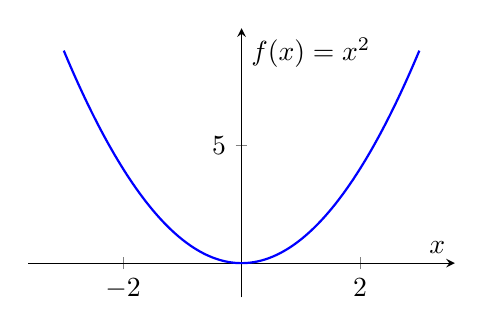
\begin{tikzpicture}
            \begin{axis}[
                axis lines = middle,
                xlabel = $x$,
                ylabel = {$f(x)=x^2$},
                xmin=-3, xmax=3,
                ymin=-0.5, ymax=9,
                samples=200,
                domain=-3:3,
                width=7cm, height=5cm,
                enlargelimits
            ]
                \addplot[blue, thick] {x^2};
            \end{axis}
        \end{tikzpicture}
        \captionof{figure}{Graphe de la fonction carré}
    \end{minipage}
    \hfill
    \begin{minipage}{0.45\textwidth}
        C'est une application : à chaque réel $x$ correspond un unique réel $f(x) = x^2$. \\
        Domaine : $\R$, Codomaine : $\R$. \\
        Image : l'ensemble des réels positifs ou nuls :
        \[
            f(\R) = \{ y \in \R \mid y \geq 0 \}.
        \]
        Quelques valeurs :
        \[
        \begin{array}{c|c|c|c|c|c}
        x & -2 & -1 & 0 & 1 & 2 \\ \hline
        f(x) & 4 & 1 & 0 & 1 & 4
        \end{array}
        \]
        On voit que $4$ est l'image de $2$ et de $-2$, et que $\sqrt{2}$ est un antécédent de $2$.
    \end{minipage}
\end{example}

% ------------------------------------------------------------------
% Image et préimage

\begin{definition}[Image et préimage]
    Soit $f : A \longrightarrow B$ une fonction.
    \begin{itemize}
        \item \textbf{L'image directe} d'un sous-ensemble $X \subset A$ par $f$ est :
        \[
            f(X) := \{ f(x) \mid x \in X \}.
        \]
        \item \textbf{La préimage} d'un sous-ensemble $Y \subset B$ par $f$ est :
        \[
            f^{-1}(Y) := \{ x \in A \mid f(x) \in Y \}.
        \]
    \end{itemize}
\end{definition}

\begin{example}
    Soit $E = \{1,2,3\}$, $F = \{a,b\}$ et $f$ définie par $f(1)=a$, $f(2)=a$, $f(3)=b$.
    \[
        f(E) = \{a,b\}, \quad f^{-1}(\{a\}) = \{1,2\}, \quad f^{-1}(\{b\}) = \{3\}.
    \]
\end{example}

% ------------------------------------------------------------------
% Composition

\begin{definition}[Composition de fonctions]
    Soient $f : E \longrightarrow F$ et $g : F \longrightarrow H$. La \emph{composition} $g \circ f : E \longrightarrow H$ est définie par :
    \[
        \forall x \in E, \quad g \circ f (x) := g(f(x)).
    \]
\end{definition}

\begin{example}
    Soient $f(x) = x^2$ et $g(x) = x+1$. Alors :
    \[
        g \circ f (x) = g(f(x)) = x^2 + 1.
    \]
\end{example}

% ------------------------------------------------------------------
% Préparation à l'injection et la surjection

\begin{remark}
    Avant d’introduire l’injectivité et la surjectivité, on peut observer que :
    \begin{itemize}
        \item Certains éléments du codomaine peuvent avoir plusieurs antécédents (ex. $4$ pour $f(x)=x^2$).
        \item Certains éléments du codomaine peuvent ne pas être atteints par la fonction (ex. $-2$ pour $f(x)=x^2$).
    \end{itemize}
    Ces observations motivent la définition des fonctions injectives et surjectives.
\end{remark}


% ==================================================================================================================================
% Injection et Surjection

\section{Injection et Surjection}

Comme nous l'avons observé avec la fonction carré, certains éléments du codomaine peuvent avoir plusieurs antécédents et certains éléments peuvent ne pas être atteints. Cela conduit naturellement aux notions d'\emph{injection}, \emph{surjection} et \emph{bijection}.

% ------------------------------------------------------------------
% Fonction injective

\subsection{Fonction Injective}

\begin{definition}[Fonction injective]
    Une fonction $f : E \longrightarrow F$ est dite \emph{injective} si des images égales impliquent des antécédents égaux. Formulée autrement :
    \[
        \forall x,y \in E, \quad f(x) = f(y) \implies x = y.
    \]
\end{definition}

\begin{remark}
    L'injectivité garantit que chaque élément de l'image provient d'un seul élément du domaine. Intuitivement, la fonction ne "fusionne" pas d'éléments distincts du domaine sur le même élément du codomaine.
\end{remark}

\begin{example}[Fonction injective]
    La fonction $f : \R_+ \longrightarrow \R$ définie par $f(x) = x^2$ est injective :
    \[
        f(2) = 4, \quad f(3) = 9, \quad f(4) = 16
    \]
    et chaque valeur de l'image correspond à un unique antécédent.
\end{example}

% ------------------------------------------------------------------
% Fonction surjective

\subsection{Fonction Surjective}

\begin{definition}[Fonction surjective]
    Une fonction $f : E \longrightarrow F$ est dite \emph{surjective} si chaque élément du codomaine est atteint par au moins un antécédent :
    \[
        \forall y \in F, \exists x \in E \text{ tel que } f(x) = y.
    \]
\end{definition}

\begin{remark}
    La surjectivité garantit que l'image couvre tout le codomaine. Intuitivement, aucun élément du codomaine n'est "laissé de côté".
\end{remark}

\begin{example}[Fonction surjective]
    La fonction $f : \R \longrightarrow \R_+$ définie par $f(x) = x^2$ est surjective, car tout réel positif possède au moins un antécédent.
\end{example}

% ------------------------------------------------------------------
% Fonction bijective

\subsection{Fonction Bijective}

\begin{definition}[Fonction bijective]
    Une fonction $f : E \longrightarrow F$ est dite \emph{bijective} si elle associe 
    à chaque élément de $F$ un unique antécédant de $E$. 
    On peut alors construire sa \emph{fonction inverse}, notée $f^{-1}$ telle que : 
        \[ f^{-1} : 
            \begin{cases}
                F \longrightarrow E \\ 
                f(x) \longmapsto x 
            \end{cases} \] 
\end{definition}

\begin{proposition}
    Pour toute fonction bijective $f : E \longrightarrow F$, on a donc : 
        \[ \forall x \in E, f^{-1}(f(x)) = x, \quad \forall y \in F, f(f^{-1}(y)) = y \] 
\end{proposition}

\begin{example}[Fonction bijective]
    La fonction $f : \R \longrightarrow \R$ définie par $f(x) = x + 1$ est bijective d'inverse. 
    \[
        f^{-1}(y) = y-1, \quad \forall y \in \R.
    \]
\end{example}

\begin{prop}[Caractérisation]
    Une fonction $f : E \longrightarrow F$ est bijective si et seulement si elle est \emph{injective} et \emph{surjective}.
\end{prop}

\begin{proposition}
    Les bijections nous permettent de faire le lien avec la théorie des ensembles. 
    En effet, deux ensembles fini $A$ et $B$ sont de même cardinal s'ils peuvent être mis en bijection. 
\end{proposition}

On peut maintenant définir la notion d'ensemble dénombrable. 

\begin{definition}[Ensemble dénombrable]
    Un ensemble $E$ est dit \emph{dénombrable} s'il peut être mis en bijection avec l'ensemble des
    entiers naturels $\N$. 
\end{definition}


